\documentclass[a4paper,12pt,twoside]{memoir}

% Castellano
\usepackage[spanish,es-tabla]{babel}
\selectlanguage{spanish}
\usepackage[utf8]{inputenc}
\usepackage[T1]{fontenc}
\usepackage{lmodern} % Scalable font
\usepackage{microtype}
\usepackage{placeins}
\usepackage{csquotes}
\usepackage{caption}
\usepackage{graphicx}
\usepackage{dirtree}

\RequirePackage{booktabs}
\RequirePackage[table]{xcolor}
\RequirePackage{xtab}
\RequirePackage{multirow}

% Links
\usepackage[colorlinks]{hyperref}
\hypersetup{
	allcolors = {red}
}

% Ecuaciones
\usepackage{amsmath}

% Rutas de fichero / paquete
\newcommand{\ruta}[1]{{\sffamily #1}}

% Párrafos
\nonzeroparskip

% Huérfanas y viudas
\widowpenalty100000
\clubpenalty100000

% Evitar solapes en el header
\nouppercaseheads

% Imagenes
\usepackage{graphicx}
\newcommand{\imagen}[2]{
	\begin{figure}[!h]
		\centering
		\includegraphics[width=0.9\textwidth]{#1}
		\caption{#2}\label{fig:#1}
	\end{figure}
	\FloatBarrier
}

\newcommand{\imagenflotante}[2]{
	\begin{figure}%[!h]
		\centering
		\includegraphics[width=0.9\textwidth]{#1}
		\caption{#2}\label{fig:#1}
	\end{figure}
}



% El comando \figura nos permite insertar figuras comodamente, y utilizando
% siempre el mismo formato. Los parametros son:
% 1 -> Porcentaje del ancho de página que ocupará la figura (de 0 a 1)
% 2 --> Fichero de la imagen
% 3 --> Texto a pie de imagen
% 4 --> Etiqueta (label) para referencias
% 5 --> Opciones que queramos pasarle al \includegraphics
% 6 --> Opciones de posicionamiento a pasarle a \begin{figure}
\newcommand{\figuraConPosicion}[6]{%
  \setlength{\anchoFloat}{#1\textwidth}%
  \addtolength{\anchoFloat}{-4\fboxsep}%
  \setlength{\anchoFigura}{\anchoFloat}%
  \begin{figure}[#6]
    \begin{center}%
      \Ovalbox{%
        \begin{minipage}{\anchoFloat}%
          \begin{center}%
            \includegraphics[width=\anchoFigura,#5]{#2}%
            \caption{#3}%
            \label{#4}%
          \end{center}%
        \end{minipage}
      }%
    \end{center}%
  \end{figure}%
}

%
% Comando para incluir imágenes en formato apaisado (sin marco).
\newcommand{\figuraApaisadaSinMarco}[5]{%
  \begin{figure}%
    \begin{center}%
    \includegraphics[angle=90,height=#1\textheight,#5]{#2}%
    \caption{#3}%
    \label{#4}%
    \end{center}%
  \end{figure}%
}
% Para las tablas
\newcommand{\otoprule}{\midrule [\heavyrulewidth]}
%
% Nuevo comando para tablas pequeñas (menos de una página).
\newcommand{\tablaSmall}[5]{%
 \begin{table}
  \begin{center}
   \rowcolors {2}{gray!35}{}
   \begin{tabular}{#2}
    \toprule
    #4
    \otoprule
    #5
    \bottomrule
   \end{tabular}
   \caption{#1}
   \label{tabla:#3}
  \end{center}
 \end{table}
}

%
% Nuevo comando para tablas pequeñas (menos de una página).
\newcommand{\tablaSmallSinColores}[5]{%
 \begin{table}[H]
  \begin{center}
   \begin{tabular}{#2}
    \toprule
    #4
    \otoprule
    #5
    \bottomrule
   \end{tabular}
   \caption{#1}
   \label{tabla:#3}
  \end{center}
 \end{table}
}

\newcommand{\tablaApaisadaSmall}[5]{%
\begin{landscape}
  \begin{table}
   \begin{center}
    \rowcolors {2}{gray!35}{}
    \begin{tabular}{#2}
     \toprule
     #4
     \otoprule
     #5
     \bottomrule
    \end{tabular}
    \caption{#1}
    \label{tabla:#3}
   \end{center}
  \end{table}
\end{landscape}
}

%
% Nuevo comando para tablas grandes con cabecera y filas alternas coloreadas en gris.
\newcommand{\tabla}[6]{%
  \begin{center}
    \tablefirsthead{
      \toprule
      #5
      \otoprule
    }
    \tablehead{
      \multicolumn{#3}{l}{\small\sl continúa desde la página anterior}\\
      \toprule
      #5
      \otoprule
    }
    \tabletail{
      \hline
      \multicolumn{#3}{r}{\small\sl continúa en la página siguiente}\\
    }
    \tablelasttail{
      \hline
    }
    \bottomcaption{#1}
    \rowcolors {2}{gray!35}{}
    \begin{xtabular}{#2}
      #6
      \bottomrule
    \end{xtabular}
    \label{tabla:#4}
  \end{center}
}

%
% Nuevo comando para tablas grandes con cabecera.
\newcommand{\tablaSinColores}[6]{%
  \begin{center}
    \tablefirsthead{
      \toprule
      #5
      \otoprule
    }
    \tablehead{
      \multicolumn{#3}{l}{\small\sl continúa desde la página anterior}\\
      \toprule
      #5
      \otoprule
    }
    \tabletail{
      \hline
      \multicolumn{#3}{r}{\small\sl continúa en la página siguiente}\\
    }
    \tablelasttail{
      \hline
    }
    \bottomcaption{#1}
    \begin{xtabular}{#2}
      #6
      \bottomrule
    \end{xtabular}
    \label{tabla:#4}
  \end{center}
}

%
% Nuevo comando para tablas grandes sin cabecera.
\newcommand{\tablaSinCabecera}[5]{%
  \begin{center}
    \tablefirsthead{
      \toprule
    }
    \tablehead{
      \multicolumn{#3}{l}{\small\sl continúa desde la página anterior}\\
      \hline
    }
    \tabletail{
      \hline
      \multicolumn{#3}{r}{\small\sl continúa en la página siguiente}\\
    }
    \tablelasttail{
      \hline
    }
    \bottomcaption{#1}
  \begin{xtabular}{#2}
    #5
   \bottomrule
  \end{xtabular}
  \label{tabla:#4}
  \end{center}
}



\definecolor{cgoLight}{HTML}{EEEEEE}
\definecolor{cgoExtralight}{HTML}{FFFFFF}

%
% Nuevo comando para tablas grandes sin cabecera.
\newcommand{\tablaSinCabeceraConBandas}[5]{%
  \begin{center}
    \tablefirsthead{
      \toprule
    }
    \tablehead{
      \multicolumn{#3}{l}{\small\sl continúa desde la página anterior}\\
      \hline
    }
    \tabletail{
      \hline
      \multicolumn{#3}{r}{\small\sl continúa en la página siguiente}\\
    }
    \tablelasttail{
      \hline
    }
    \bottomcaption{#1}
    \rowcolors[]{1}{cgoExtralight}{cgoLight}

  \begin{xtabular}{#2}
    #5
   \bottomrule
  \end{xtabular}
  \label{tabla:#4}
  \end{center}
}


\graphicspath{ {./img/} }

% Capítulos
\chapterstyle{bianchi}
\newcommand{\capitulo}[2]{
	\setcounter{chapter}{#1}
	\setcounter{section}{0}
	\chapter*{#2}
	\addcontentsline{toc}{chapter}{#1. #2}
	\markboth{#2}{#2}
}

% Apéndices
\renewcommand{\appendixname}{Apéndice}
\renewcommand*\cftappendixname{\appendixname}

\newcommand{\apendice}[1]{
	%\renewcommand{\thechapter}{A}
	\chapter{#1}
}

\renewcommand*\cftappendixname{\appendixname\ }

% Formato de portada
\makeatletter
\usepackage{xcolor}
\newcommand{\tutor}[1]{\def\@tutor{#1}}
\newcommand{\course}[1]{\def\@course{#1}}
\definecolor{cpardoBox}{HTML}{E6E6FF}
\def\maketitle{
  \null
  \thispagestyle{empty}
  % Cabecera ----------------
\begin{center}%
	{\noindent\Huge Universidades de Burgos, León y Valladolid}\vspace{.5cm}%
	
	{\noindent\Large Máster universitario}\vspace{.4cm}%
	
	{\noindent\Huge \textbf{Inteligencia de Negocio y Big~Data en Entornos Seguros}}\vspace{.4cm}%
\end{center}%

\begin{center}%
	
\includegraphics[height=3cm]{img/escudoUBU} \hspace{1cm}
	
\includegraphics[height=3cm]{img/escudoUVA} \hspace{1cm}
	
\includegraphics[height=3cm]{img/escudoULE} \vspace{1cm}%
\end{center}%

  \vfill
  % Título proyecto y escudo informática ----------------
  \colorbox{cpardoBox}{%
    \begin{minipage}{.9\textwidth}
      \vspace{.0cm}\Large
      \begin{center}
      \textbf{Trabajo Fin de Máster}\vspace{.4cm}\\
      \textbf{\LARGE\@title{}}
      \end{center}
      \vspace{.1cm}
    \end{minipage}

  }%
  \hfill
  \vfill
  % Datos de alumno, curso y tutores ------------------
  \begin{center}%
  {%
    \noindent\LARGE
    Presentado por \@author{}\\ 
    en Universidad de Burgos --- \@date{}\\
    Tutores: \@tutor{}\\
  }%
  \end{center}%
  \null
  \cleardoublepage
  }
\makeatother

\newcommand{\nombre}{Ismael Franco Hernando} %%% cambio de comando

% Datos de portada
\title{Aplicación de Machine Learning a imágenes 1D y 2D de control de calidad en recubrimiento de Zinc}
\author{\nombre}
\tutor{Carlos Enrique Vivaracho Pascual \\\phantom{Turi: }Joaquín B. Ordieres Meré}
\date{\today}

\begin{document}

\maketitle


\newpage\null\thispagestyle{empty}\newpage


%%%%%%%%%%%%%%%%%%%%%%%%%%%%%%%%%%%%%%%%%%%%%%%%%%%%%%%%%%%%%%%%%%%%%%%%%%%%%%%%%%%%%%%%
\thispagestyle{empty}


\noindent
\begin{center}%
	{\noindent\Huge Universidades de Burgos, León y Valladolid}\vspace{.5cm}%
	
\begin{center}%
	
\includegraphics[height=3cm]{img/escudoUBU} \hspace{1cm}
	
\includegraphics[height=3cm]{img/escudoUVA} \hspace{1cm}
	
\includegraphics[height=3cm]{img/escudoULE} \vspace{1cm}%
\end{center}%

	{\noindent\Large \textbf{Máster universitario en Inteligencia de Negocio y Big~Data en Entornos Seguros}}\vspace{.5cm}%
\end{center}%



\noindent D. nombre tutor, profesor del departamento de nombre departamento, área de nombre área.

\noindent Expone:

\noindent Que el alumno D. \nombre, con DNI 71363577M, ha realizado el Trabajo final de Máster en Inteligencia de Negocio y Big Data en Entornos Seguros 
          titulado Aplicación de Machine Learning a imágenes 1D y 2D de control de calidad en recubrimiento de Zinc. 

\noindent Y que dicho trabajo ha sido realizado por el alumno bajo la dirección del que suscribe, en virtud de lo cual se autoriza su presentación y defensa.

\begin{center} %\large
En Burgos, {\large \today}
\end{center}

\vfill\vfill\vfill

% Author and supervisor
\begin{minipage}{0.45\textwidth}
\begin{flushleft} %\large
Vº. Bº. del Tutor:\\[2cm]
D. nombre tutor
\end{flushleft}
\end{minipage}
\hfill
\begin{minipage}{0.45\textwidth}
\begin{flushleft} %\large
Vº. Bº. del co-tutor:\\[2cm]
D. nombre co-tutor
\end{flushleft}
\end{minipage}
\hfill

\vfill

% para casos con solo un tutor comentar lo anterior
% y descomentar lo siguiente
%Vº. Bº. del Tutor:\\[2cm]
%D. nombre tutor


\newpage\null\thispagestyle{empty}\newpage




\frontmatter

% Abstract en castellano
\renewcommand*\abstractname{Resumen}
\begin{abstract}
En el proceso de galvanizado es muy importante mantener los niveles de la capa de zinc entre unos mínimos, para garantizar que el acero aguante los diferentes escenarios para los que esté dedicado, y unos máximos, para evitar que la empresa pierda dinero al gastar demás de zinc y evitar que el acero se endurezca demasiado evitando que se pueda trabajar con él.

Una empresa dedicada a este proceso, nos ha solicitado que creemos un modelo que, a través de datos medidos por sensores en la cadena de producción, y aplicado sobre bobinas que tiene algún defecto, se realice una predicción sobre si la bobina podrá ser aprovechable o no.

Para ello, se llevarán a cabo diversos experimentos sobre datos 1D y 2D, para ver cuál de ellos da mejores resultados junto con la validación cruzada, probando diversos parámetros para obtener el mejor resultado posible.

Además, se llevará a cabo una aplicación que simulará el proceso que un operario de la empresa debería de seguir para cargar los datos de las bobinas y esperar las predicciones sobre los mismos.
\end{abstract}

\renewcommand*\abstractname{Descriptores}
\begin{abstract}
Galvanizado, bobinas galvanizadas, \emph{deep learning}, redes neuronales convolucionales, investigación, predicción bobinas, validación cruzada.
\end{abstract}

\clearpage

% Abstract en inglés
\renewcommand*\abstractname{Abstract}
\begin{abstract}
In the galvanizing process, it is crucial to maintain zinc layer levels within certain minimums to ensure that the steel withstands different scenarios it is intended for, as well as maximums to prevent the company from losing money by overspending on zinc and avoid excessive hardening of the steel, making it difficult to work with.

A company dedicated to this process has requested us to create a model that, using data measured by sensors in the production line and applied to coils with some defect, can make a prediction on whether the coil will be usable or not.

To achieve this, various experiments will be conducted on 1D and 2D data to determine which of them yields better results, along with cross-validation, while testing different parameters to obtain the best possible outcome.

Additionally, an application will be developed to simulate the process that a company operator should follow to load coil data and wait for the predictions on them.
\end{abstract}

\renewcommand*\abstractname{Keywords}
\begin{abstract}
Galvanized, galvanized coils, deep learning, convolutional neural networks, research, coil prediction, cross-validation.
\end{abstract}

\clearpage

% Indices
\tableofcontents

\clearpage

\listoffigures

\clearpage

\listoftables
\clearpage

\mainmatter

\part*{Memoria}
\addcontentsline{toc}{part}{Memoria}


\capitulo{1}{Introducción}

Descripción del contenido del trabajo y del estrucutra de la memoria y del resto de materiales entregados.

\capitulo{2}{Objetivos del proyecto}

Este apartado explica de forma precisa y concisa cuales son los objetivos que se persiguen con la realización del proyecto. Se puede distinguir entre los objetivos marcados por los requisitos del software a construir y los objetivos de carácter técnico que plantea a la hora de llevar a la práctica el proyecto.

\capitulo{3}{Trabajos relacionados}

Analizando trabajos que también usen el \emph{deep learning} en la rama de la industria centrada en el acero galvanizado, existe una gran variedad de artículos centrados en este tema; lo que afirma la importancia de controlar los niveles de zinc en el acero, comentado previamente en la introducción. 

Pese a todo, el número de artículos centrados en los mismos objetivos que este proyecto es bastante limitado, ya que la mayoría busca predecir las capas de zinc de láminas de acero con redes neuronales. A continuación se muestran dos artículos, cuyo principal objetivo es predecir las capas de zinc del acero galvanizo, a partir de diferentes medidas tomadas en la línea de producción.

\section{Research on Zinc Layer Thickness Prediction Based on LSTM Neural Network}
Autores: Zhao Lu, Yimin Liu y Shi Zhong

Este artículo \cite{9602402} utiliza una red neuronal LSTM (\emph{Long Short-Term Memory}), que es un tipo de red recurrente (y que en el siguiente punto se explicará más en detalle), que permite detectar propiedades de los datos a lo largo del tiempo gracias a su capacidad de retener memoria.

El propósito de dicho artículo es el de predecir el espesor del zinc de acero galvanizado en caliente, con el fin de ver si cumple con los requisitos mínimos y máximos necesarios. Para ello se emplearán los diferentes datos medidos por los sensores en la cadena de producción, y, en última instancia, se realizará la predicción.

Finalmente, los resultados obtenidos son muy buenos, ya que su error porcentual absoluto es del 1.824\% y teniendo en cuenta que las capas de zinc se miden en micras, son un valor muy bueno debido a la alta precisión que se necesita tener.

\section{Coating Thickness Modeling and Prediction for Hot-dip Galvanized Steel Strip Based on GA-BP Neural Network}
Autores: Kai Mao, Yong-Li Yang, Zhe Huang y Dan-yang Yang

Este segundo artículo \cite{9164854} es muy parecido al anterior, solo que utilizan una red neuronal BP (\emph{Back Propagation}), que se caracteriza por ser una red que puede ajustar con el paso del tiempo los pesos de sus enlaces con el fin de reducir al máximo la función de error.

El principal objetivo del artículo es predecir el espesor de zinc sobre chapas de acero galvanizadas en caliente. Para ello, usarán diferentes parámetros medidos durante el proceso de galvanizado, como la velocidad de la línea, la presión de la chapa que corta el acero o la temperatura a la que se encuentra el zinc.

Finalmente, se comenta que los resultados de la red neuronal BP no son demasiado buenos, por lo que se añadió también un algoritmo genético que permitió optimizar la red, y con ello obtener buenos resultados; comentando incluso que es posible su uso por parte de las empresas en la fase de control de calidad.


\capitulo{4}{Conceptos teóricos}

\section{Machine Learning y Deep Learning}
El proyecto se ha basado en el uso del \emph{machine learning}, y más en concreto, en una de sus ramas: el \emph{deep learning}.

\subsection{Machine Learning}
El aprendizaje automático, también conocido como \emph{machine learning} en inglés, \cite{bobadilla2021machine} se centra en conseguir que con unos datos iniciales, y aplicado algún tipo de algoritmo o técnica, un computador sea capaz de aprender.

Para conseguir esto, adopta el proceso de observación y aprendizaje utilizado por los seres vivos, de forma que cuantos más ``sucesos'' haya, mayor conocimiento podrá obtener, es decir, cuanto mayor sea el número de datos con el que se cuente, los resultados obtenidos también serán mejores. En la Figura \ref{f:esquemaML} se puede ver detalladamente como funciona el \emph{machine learning}.

\begin{figure}[h]
    \centering
    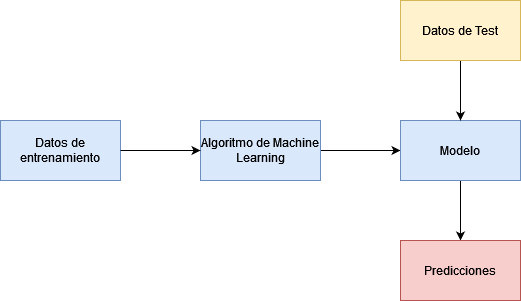
\includegraphics[scale=0.7]{img/Esquema_ML.png}
    \caption{Esquema Algoritmos Machine Learning (Realización Propia).}
    \label{f:esquemaML}
\end{figure}

Este tipo de aprendizaje debe utilizarse en problemas donde se tengan multitud de datos y multitud de escenarios y posibilidades, y que a su vez se puedan modelar todas sus soluciones de forma matemática.

Finalmente, los tipos de \emph{machine learning}, según el problema al que se enfrente, son:
\begin{itemize}
    \item \textbf{Aprendizaje supervisado:} cada dato del conjunto de datos va acompañado de la clase a la que pertenece.
    \item \textbf{Aprendizaje no supervisado:} se desconoce la clase a la que pertenece cada dato.
    \item \textbf{Aprendizaje semisupervisado:} en el conjunto de datos, se conocerá la clase de alguno de los datos, mientras que de otros no.
    \item \textbf{Aprendizaje por refuerzo:} el algoritmo aprende en base a sus aciertos y fallos, mediante un sistema de recompensas y penalizaciones.
\end{itemize}

\subsection{Deep Learning}
El aprendizaje profundo, también conocido como \emph{deep learning} en inglés, \cite{bobadilla2021machine} es una de las ramas del \emph{machine learning} que se basa en el sistema nervioso humano, donde las neuronas están conectadas entre sí y cada una de ellas se encarga de una tarea en específico.

Esta estructura permite que ciertas zonas se encarguen de detectar ciertos patrones o características de los datos, lo que permite una gran mejoría con respecto al \emph{machine learning}, ya que esta estructura otorga a la red la posibilidad de aprender de manera automática, además de conseguir mejoras de rendimiento.

\section{Redes Neuronales Artificiales}
Las redes neuronales artificiales \cite{izaurieta2000redes} buscan recrear el sistema nervioso del ser humano, donde existen multitud de neuronas conectadas entre sí, y que intercambian pulsos.

En una red neuronal artificial existen multitud de neuronas artificiales conectadas entre sí por un enlace, que habitualmente suele llevar un peso asociado, consiguiendo así que otra neurona se active según el pulso que le llegue por sus enlaces.

Durante el proceso de entrenamiento, y de manera iterativa, se van modificando estos pesos, buscando los valores óptimos que minimicen alguna función de error o pérdida. Es la forma en la que red ``aprende'' a partir de los datos que se le prestan.

Según como fluyan los datos en la red, se distinguen principalmente dos tipos:
\begin{itemize}
    \item \textbf{Red neuronal prealimentada:} los datos siempre van hacia delante pasando por diferentes capas hasta llegar a la capa de salida. Durante todo este proceso no se permiten ni bucles ni volver hacia atrás, es decir, la información siempre se mueve hacia la siguiente capa. La Figura \ref{f:redneuronal} muestra de una manera más gráfica cómo se mueve la información. Este tipo de red es el más básico y se usa principalmente en problemas de clasificación y regresión.
    \item \textbf{Red neuronal recurrente:} permite que a lo largo de la red haya bucles o que se pueda avanzar hacia una capa anterior, otorgando a las neuronas una memoria interna que permitirá ir adaptándose según lleguen nuevos datos. Es por ello que se utiliza principalmente en problemas con datos secuenciales o \emph{data stream}.
    
\end{itemize}
\begin{figure}[h]
 \centering
  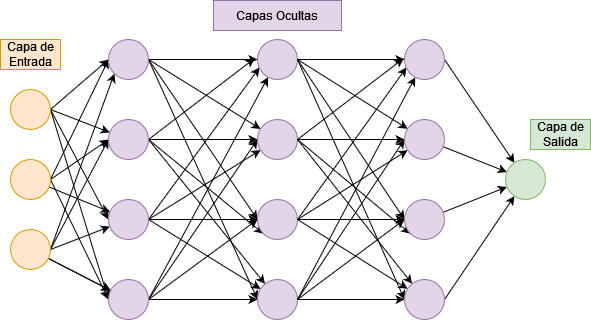
\includegraphics[width=0.8\textwidth]{img/RedNeuronal.png}
 \caption{Ejemplo Red Neuronal Artificial (Realización Propia)}
 \label{f:redneuronal}
\end{figure}

\subsection{Redes Neuronales Convolucionales}
Las redes neuronales convolucionales \cite{prieto2019redes}, también conocidas como CNN (por sus siglas en inglés \emph{Convolutional Neural Network}), son la variante de las redes neuronales artificiales más extendidas y utilizadas en la actualidad. Esto se debe al gran rendimiento que se obtiene en aquellos casos donde los datos se encuentren en cuadrícula, como un \emph{array} o matriz. Sus principales usos son en la clasificación de imágenes o en la detección de objetos. Es por ello, que, pesé a que existan muchas más variantes de redes neuronales, se ha empleado este tipo durante el desarrollo del proyecto. 

Este tipo de red se basa en aplicar dos operaciones diferentes: convolución y \emph{pooling}.

\subsubsection{Convolución}
La convolución \cite{prieto2019redes} es una operación que busca obtener características de los datos para que puedan ser aprendidos por la red neuronal. Para ello se utiliza una matriz, comúnmente denominada \emph{kernel}, que recorre todas las celdas de los valores de entrada y calcula, junto con las celdas de su alrededor, el producto escalar y dicho valor se almacena en el \emph{kernel}. De esta forma se va completando, y obteniendo una matriz, generalmente, de un tamaño menor que el de los datos de entrada.

En la Figura \ref{f:convo} se puede ver como funciona esta operación usando un \emph{kernel} de tamaño 3x3 sobre los datos iniciales.

\begin{figure}[h]
 \centering
  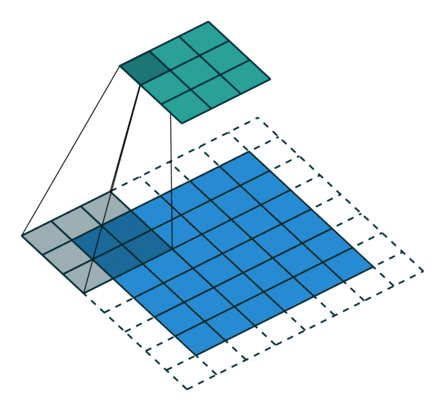
\includegraphics[width=0.6\textwidth]{img/Convo.png}
 \caption{Operación de Convolución \cite{wiki:convo}}
 \label{f:convo}
\end{figure}

\subsubsection{Pooling}
La operación \emph{pooling} \cite{prieto2019redes} busca reducir la dimensionalidad de la matriz de características obtenida en la operación anterior, de forma que queden aquellas más relevantes y se disminuya la carga computacional de la red neuronal.

Para ello, se divide el \emph{kernel} en una malla de un tamaño en específico, en la que, para cada celda, se devuelve un valor, que habitualmente suele ser el valor máximo o el valor medio; ya que según el problema a resolver puede ser mejor solución el uso del valor máximo, puesto que resalta las características más importantes, o el valor medio, que devuelve el promedio de las características.

En la Figura \ref{f:pooling} se puede observar un ejemplo de \emph{pooling} aplicando una malla de 2x2 y devolviendo por cada celda el valor máximo.

\begin{figure}[h]
 \centering
  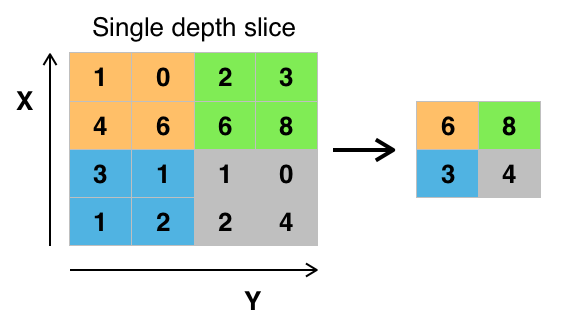
\includegraphics[width=0.7\textwidth]{img/pooling.png}
 \caption{Operación de \emph{Pooling} \cite{wiki:pooling}}
 \label{f:pooling}
\end{figure}

\section{Conjunto de Datos Desbalanceado}
En problemas de clasificación, cuando se quiere construir un modelo aplicando \emph{deep learning} es importante contar con una gran cantidad de datos de cada una de las clases. Aunque esto es, en algunos casos, difícil, por ejemplo, en medicina es más común que la gente este sana a que la gente esté enferma, por lo que en este conjunto de datos sería difícil de tener un número de personas equilibrado de ambas clases o el número de muestras equitativo de ambas clases sería limitado. A esto se le conoce como conjunto de datos desbalanceado o desequilibrado.

Ante estos inconvenientes, suele ser recomendable y eficiente aplicar alguna de las tres estrategias siguientes \cite{Na8_2020}:
\begin{itemize}
    \item \textbf{Submuestreo:} consiste en reducir el número de datos de la clase mayoritaria para tener ambas clases con el mismo número de registros.
    \item \textbf{Sobremuestreo:} se basa en generar nuevos datos de la clase minoritaria para poder equilibrar los datos de cada clase. Estos datos pueden ser repitiendo los mismos datos o creando nuevos ``sintéticos'', ya que según el problema puede ser mejor utilizar una técnica u otra.
    \item \textbf{Sobremuestreo y submuestreo}: se aplica en primer lugar el sobremuestreo para equilibrar ambas clases, y a continuación, aplicar el submuestreo sobre todos los datos para eliminar aquellos que estén repetidos o sean muy similares.
\end{itemize}


\capitulo{5}{Técnicas y herramientas}

Este punto muestra las diferentes técnicas  y herramientas que se han utilizado en el proyecto. Además, también incluye la metodología y gestión seguida en la construcción del proyecto.

\section{Metodología}
Durante el desarrollo del proyecto se ha empleado la metodología ágil del \emph{Scrum}. En dicha metodología se pretende realizar las diferentes tareas de manera incremental, formando un \emph{sprint}. Estos últimos tenían una duración de dos semanas, donde al pasar el tiempo se llevaba a cabo una reunión para revisar el progreso y tomar las decisiones adecuadas en el correcto desarrollo del proyecto.

Con respecto al entendimiento y procesado de los datos se ha seguido la metodología CRISP-DM, es decir, se han realizado diferentes etapas (entendimiento, preparación, modelado, evaluación y despliegue) con el conjunto de datos original.

\section{Gestión del Proyecto}
\subsection{GitHub}
\emph{GitHub}\footnote{GitHub: \url{https://github.com/}} es un servicio que permite alojar los proyectos de manera remota, e ir subiendo las nuevas versiones que se desarrollen de manera que se pueda llevar un control de las diferentes versiones, con sus cambios y mejoras.

\section{Herramientas}
\subsection{Anaconda}
\emph{Anaconda}\footnote{Anaconda: \url{https://www.anaconda.com/}} es una distribución de uso libre y abierta basada en \emph{Python} y cuyo principal uso es en las ramas de ciencias de datos y en aprendizaje automático.

\subsection{Jupyter Notebook}
\emph{Jupyter Notebook}\footnote{Jupyter Notebook: \url{https://jupyter.org/}} es una interfaz web utilizada principalmente para ejecutar sentencias de código desde el navegador a través de los \emph{notebooks} que permite generar.

\section{Bibliotecas de Python}
Durante todo el desarollo del proyecto se ha utilizado el lenguaje de programación \emph{Python} en diferentes \emph{notebooks}. Las bibliotecas que se han empleado durante el desarrollo han sido las siguientes.

\subsection{Pandas}
La librería \emph{Pandas}\footnote{Pandas: \url{https://pandas.pydata.org/}} permite manipular y analizar grandes cantidades de datos. Se asemeja mucho a la herramienta de \emph{Excel} pero en \emph{Python}.

\subsection{NumPy}
\emph{NumPy}\footnote{NumPy: \url{https://numpy.org/}} permite utilizar arrays y matrices sobre las cuales realizar las principales operaciones matemáticas. Además, son muy útilies frente a grandes conjuntos de datos, ya que las operaciones están muy optimizadas.

\subsection{MySQL}
La librería \emph{MySQL}\footnote{MySQL: \url{https://www.mysql.com/}} permite conectarse a una base de datos \emph{MySQL} desde \emph{Python}. Además, permite realizar las principales operaciones en una base de datos tradicional: consultas y añadir o eliminar datos.

\subsection{PyMySQL}
La librería \emph{PyMySQL} es muy similar a la anterior, solo que permite llevar a cabo operaciones en bases de datos de forma mucho más amigable por parte del usuario.

\subsection{TensorFlow}
\emph{TensorFlow}\footnote{TensorFlow:\url{https://www.tensorflow.org}} es una librería desarrollada por \emph{Google} y que se centra principalmente en el uso del aprendizaje automático y la inteligencia artificial. Siendo el primer caso, el utilizado en este proyecto, para poder configurar y crear modelos de aprendizaje automático.

Además, incluye \emph{Keras}\footnote{Keras:\url{https://keras.io/}} lo que simplifica y facilita la construcción de redes neuronales.

\subsection{Scikit-Learn}
La librería \emph{Scikit-learn}\footnote{Scikit-learn:\url{https://scikit-learn.org/}} se centra en el aprendizaje automático, incluyendo los principales algoritmos de clasificación y regresión. Además, incluye alguna herramienta que permite valorar los resultados obtenidos con el modelo, siendo este punto la principal utilidad en el proyecto.

\subsection{Imbalanced-Learn}
\emph{Imbalanced-learn}\footnote{Imbalanced-learn:\url{https://imbalanced-learn.org/}} se centra en abordar el problema de clases desbalanceadas, de modo que tiene múltiples herramientas para intentar de solventar este inconveniente.

\subsection{Matplotlib}
\emph{Matplotlib}\footnote{Matplotlib: \url{https://matplotlib.org/}} permite generar los gráficos más habituales en dos dimensiones, además, estas pueden ser interactivas o dinámicas, facilitando así la comprensión por parte del usuario.

\subsection{Jupyter Widgets}
\emph{Jupyter Widgets}\footnote{Jupyter Widgets: \url{https://github.com/jupyter-widgets/ipywidgets}} otorga a los \emph{notebooks} un cierto dinamismo e interactividad al usuario, de forma que los \emph{notebooks} no queden tan estáticos, y que no suponga únicamente ejecutar celdas sin apenas interacción por parte del usuario.

\section{Documentación}
\subsection{\LaTeX}
\LaTeX\footnote{\LaTeX: \url{https://www.latex-project.org/}} es un sistema de composición de textos usado principalmente en la escritura de textos con alta calidad tipográfica. 

\subsection{Overleaf}
\emph{Overleaf}\footnote{Overleaf: \url{https://www.overleaf.com/}} es un editor colaborativo de \LaTeX{} cuyo principal uso es escribir, editar y publicar documentos científicos, todo ello gestionado desde la nube.

\subsection{Draw.io}
\emph{Draw.io}\footnote{Draw.io: \url{https://app.diagrams.net/}} es una herramienta web que permite, entre otras cosas, crear diagramas, por lo que se ha empleado principalmente para representar pequeños esquemas o diagramas UML.

\subsection{Tables Generator}
\emph{Tables Generator}\footnote{Tables Generator: \url{https://www.tablesgenerator.com/\#}} es una web que facilita la creación de tablas para \LaTeX, ya que se pueden diseñar a través de una interfaz y posteriormente exportarlo a código.


\capitulo{6}{Aspectos relevantes del desarrollo del proyecto}

Este punto es el más importante de la memoria, ya que contiene, de manera descriptiva y detallada, el proceso seguido desde el inicio hasta el fin del proyecto. Para una mejor comprensión, el orden de los subpuntos que contiene este apartado están ordenados de manera cronológica. Además, se hablará acerca de los problemas surgidos, soluciones tomadas y alguna posible alterativa. 

Antes de entrar en materia, cabe destacar que la primera idea que teníamos por parte de la empresa, es que querían comprobar, si con los niveles mínimos y máximos de zinc, la decisión por parte del operario era la correcta acerca de si la bobina era válida o no. Y tras comprobar los niveles y clasificar de nuevo las bobinas, crear una red neuronal capaz de clasificar futuras bobinas.

Pero más adelante se nos comentó que las decisiones por parte del operario sobre si la bobina era válida o no, eran las correctas, y su interés estaba en obtener un modelo que con los valores capturados por los sensores se pueda predecir, sin necesidad del operario, si la bobina es correcta o no.

\section{Carga de Datos y Evaluación de Bobinas}
En esta primera fase, lo primero que se hizo fue cargar los datos que nos había cedido la empresa, y que se encontraban en una base de datos de MySQL, para realizar una sencilla exploración de datos y saber con exactitud el número de datos con el que se contaba.

Antes de nada, comentar que la empresa nos cedió datos de bobinas medidas por sensores 1D y 2D, por lo que se cuenta con dos tipos de datos. Además, de los sensores 1D se contaba con dos parejas de sensores diferentes (cada pareja tenía un sensor que media la capa de arriba y otro la capa de abajo de la bobina.) De manera gráfica se entiende muy fácilmente cómo son los datos con los que se cuenta. En la Figura \ref{f:datos1D}se puede ver como son los datos 1D, que no dejarían de ser más que un \emph{array} de una dimensión. Con respecto a los datos 2D, Figura \ref{f:datos2D}, se pueden interpretar como una matriz de 9 filas y el número de columnas cambiantes según cada bobina. Además, a cada celda, tanto en datos 1D como 2D, se le conoce como teja.

\begin{figure}[h]
 \centering
  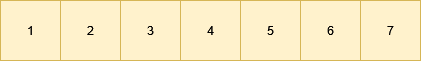
\includegraphics[width=0.9\textwidth]{img/1D.png}
 \caption{Ejemplo estructura datos 1D}
 \label{f:datos1D}
\end{figure}

\begin{figure}[h]
 \centering
  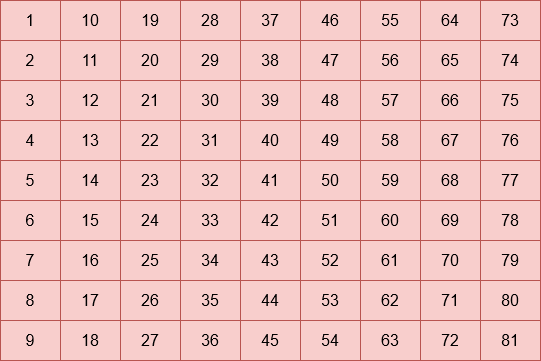
\includegraphics[width=0.9\textwidth]{img/2D.png}
 \caption{Ejemplo estructura datos 2D}
 \label{f:datos2D}
\end{figure}




Una vez explicada la estructura de los diferentes datos, añadir que se cuentan 1160 bobinas previamente evaluadas por un operario, con 115972 registros de los datos 1D, correspondientes a las diferentes tejas medidas, y con 127312 registros de los datos 2D.

Ahora que ya se comprendían los datos, era turno de evaluar cada bobina. Para ello se creó una función que evaluaba cada bobina con sus diferentes tejas y se comprobaba que en cada una de ellas se cumplían con los requisitos mínimos y máximos de zinc correspondientes a la bobina. Toda esta evaluación se realizaba para cada uno de los sensores, y además, se contaban el número de fallos, es decir, el número de tejas que no cumplía los requisitos, y si se había producido algún calibrado. Esto último consiste en reiniciar los sensores y sus mediciones serían 0 en ese registro, pero que no indica que la teja este mal. 

En la Figura \ref{f:evalua1} se muestra el resultado obtenido para las dos primeras bobinas, en las que se indica la ID de la bobina (\emph{COILID}), la ID del sensor (\emph{MID}), la clase del operario y la clase obtenida por el proyecto, y finalmente el número de fallos y el número de calibrados, si es que se ha producido alguno.

\begin{figure}[h]
 \centering
  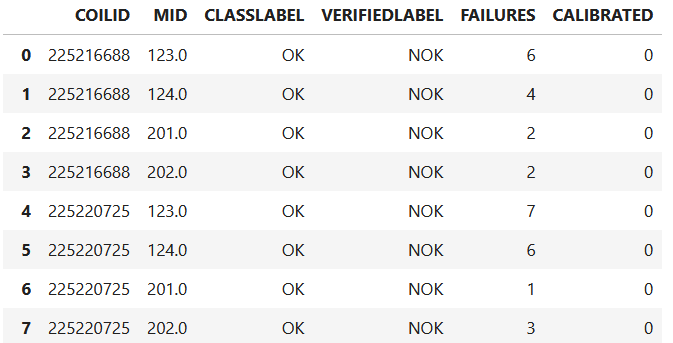
\includegraphics[width=0.9\textwidth]{img/evalua1.PNG}
 \caption{Ejemplo de Evaluación de 2 Bobinas}
 \label{f:evalua1}
\end{figure}

Finalmente, en esta fase se mostraron las estadísticas de las clases obtenidas por los operarios y por el proyecto. A continuación, se puede ver en detalle:
\begin{verbatim} 
        Los valores de los operarios han sido:
         OK    3340
        NOK    1300
        
        Los valores que se han obtenido son:
         OK      98
        NOK    4542
\end{verbatim}
A simple vista se puede observar que había una anomalía, y como ya se había comentado previamente, se debía a esa pequeña confusión que hubo en un primer lugar con la empresa, y que tras una nueva reunión, se dijo que estas bobinas sí que estaban ya bien clasificadas previamente por un operario y que simplemente era necesario proceder a la construcción de una red neuronal. 

También se puede ver como el conjunto de datos está desbalanceado (mirando las estadísticas de las clases de los operarios), ya que la clase OK es la mayoritaria, con aproximadamente un 72\% de los datos, mientras que la clase NOK es la minoritaria con aproximadamente el 28\% de los datos.

\section{Visualización de las Bobinas}
En esta segunda fase, se realizó la parte correspondiente a representar gráficamente los datos 1D junto con los valores en los que tiene que encontrarse el zinc. Para ello, se realizó un desplegable con las IDs de las diferentes bobinas, y que al seleccionar una, se mostraran los gráficos de los cuatro sensores. 

La Figura \ref{f:visu} muestra un ejemplo de visualización de las cuatro gráficas, correspondientes a los diferentes sensores, junto con los diferentes valores de zinc medidos; además de una línea roja que representa el máximo o el mínimo de zinc en cada caso.

\begin{figure}[h]
 \centering
  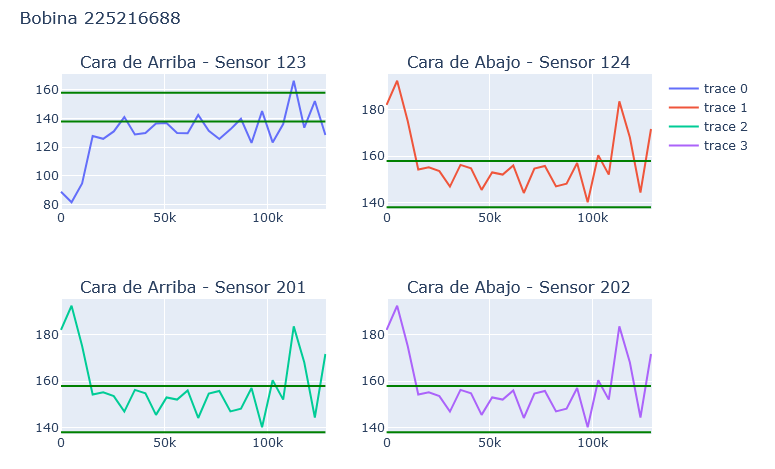
\includegraphics[width=0.9\textwidth]{img/visuaBobi.PNG}
 \caption{Ejemplo de Visualización para una Bobina}
 \label{f:visu}
\end{figure}

\section{Obtención de las Características de las Bobinas}
Esta tercera fase se ha centrado en la obtención de las principales \emph{features} de cada bobina, junto con la codificación del mapa que forman los datos 1D o 2D, para posteriormente ser utilizados en la red neuronal. 

En primer lugar, las características o \emph{features} que se han obtenido para cada bobina han sido las siguientes:
\begin{itemize}
    \item \textbf{ZNMAX\_FAILURES:} se corresponde al número de tejas que tiene una capa de zinc superior al estipulado. Los fallos se contarán desde que hay un fallo hasta que se encuentra una teja correcta, no un fallo por cada teja con un defecto.
    \item \textbf{ZNMIN\_FAILURES:} es el número de tejas de la bobina que tiene menos zinc del mínimo estipulado. Los fallos también se cuentan con el mismo criterio que el caso anterior.
    \item \textbf{CALIBRATED:} se corresponde al número de tejas en las que se ha producido un calibrado (reinico de los sensores).
    \item \textbf{TOTAL\_TILEID:} indica el número total de las tejas que tiene la bobina.
    \item \textbf{L\_DIS:} contiene el número de tejas que hay desde el inicio de la bobina hasta el último fallo antes de la mitad de la bobina.
    \item \textbf{R\_DIS:} indica el número de tejas que hay desde el fallo más cercano a la mitad y el final.
\end{itemize}

En segundo lugar, la codificación del mapa de las bobinas se ha llevado de la siguiente manera:
\begin{itemize}
    \item \textbf{1:} en caso de que la teja tenga más zinc del máximo.
    \item \textbf{0:} indica que el valor de zinc de la teja está dentro de los mínimos y máximos.
    \item \textbf{-1:} correspondiente a una teja que tenga menos zinc del mínimo necesario.
\end{itemize}

Cabe destacar que, tanto las \emph{features} como la codificación del mapa de la bobina son iguales tanto para los datos 1D como 2D. Para visualizarlo mejor, la Figura \ref{f:fea1d}, muestra un ejemplo de salida de datos 1D. En ella se pueden ver todos los atributos anteriormente mencionados para una misma bobina y los valores obtenidos por parte de los 4 sensores diferentes.

\begin{figure}[h]
 \centering
  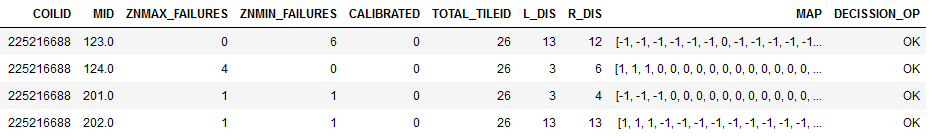
\includegraphics[width=1\textwidth]{img/fea1D.PNG}
 \caption{Ejemplo de características obtenidas para datos 1D}
 \label{f:fea1d}
\end{figure}

Por otro lado, tenemos la Figura \ref{f:fea2d}, que muestra, para la misma bobina que en la Figura anterior, las características obtenidas para los sensores 2D. En dicha figura, se puede ver como el mapa es también un \emph{array}, ya que por comodidad se ha guardado así, pero posteriormente, cuando se lea, se reconstruirá en forma de matriz.

\begin{figure}[h]
 \centering
  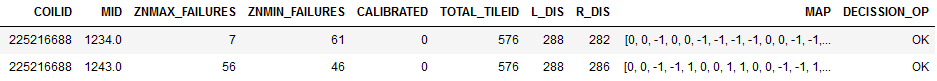
\includegraphics[width=1\textwidth]{img/fea2D.PNG}
 \caption{Ejemplo de características obtenidas para datos 2D}
 \label{f:fea2d}
\end{figure}

Finalmente, en esta tercera fase, se han guardado las características obtenidas de los datos 1D y 2D en una base de datos. Para ello se han creado dos tablas, FEATURES\_1D y FEATURES\_2D, donde se almacena todo el contenido previamente calculado.

\section{Pruebas CNNs}
Una vez se contaba con los datos preparados, en este cuarta fase se realizaron diferentes pruebas en la construcción de CNNs de la librería \emph{TensorFlow}, con el fin de poder familiarizarse con su uso. Además, y antes de empezar a construir redes neuronales, había que preprocesar los datos para poder usarlos. También, indicar que en esta fase las pruebas fueron únicamente con datos 1D.

En primer lugar, se cargaron los mapas codificados de las bobinas 1D, obtenidos en la tercera fase, y se decidió unir en un único \emph{array} cada par de sensores, es decir, unir los mapas de los sensores 123 y 124 y, por otro lado, los sensores 201 y 202, con el fin de poder utilizar las convoluciones 1D sobre los datos.

A continuación, sobre estos nuevos mapas unidos, se aplicó la técnica de \emph{padding}, que se basa en rellenar los datos con un valor para que todos ellos tengan las mismas dimensiones, ya que es necesario para las redes neuronales que se van a construir. En este caso, se rellenaron los datos con 0, hasta que todos los datos tuvieran una longitud de 208, puesto que fue el valor más grande encontrado dentro del conjunto de datos.

Ahora ye se contaba con los mapas preparados para ser usados, pero antes había que transformar la clase de \emph{string} a \emph{int}. Dicha transforamción fue: un 0 para la clase OK y un 1 para la clase NOK.

En este punto ya se cuenta con los datos listos, por lo que era turno de construir modelos. En primer lugar, se crearon modelos individuales para aprender como funciona su construcción, la Figura \ref{f:modelo1}, muestra un ejemplo de construcción. Aunque, como suele ser habitual en estos casos para generar modelos, se utilizará la estrategia de validación cruzada  o \emph{cross validation} para poder evaluar los diferentes modelos construidos de manera más precisa y robusta.

\begin{figure}[h]
 \centering
  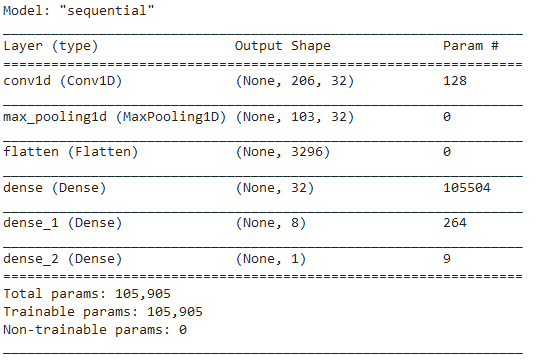
\includegraphics[width=0.8\textwidth]{img/modelo1.PNG}
 \caption{Ejemplo de Construcción de Modelo}
 \label{f:modelo1}
\end{figure}

Finalmente, en esta fase de pruebas también se decide hacer pruebas utilizando alguna técnica para ajustar el conjunto de datos desbalanceado. En este caso se opta, debido al bajo número de registros, a realizar un sobremuestreo de los datos, y más concretamente aplicar la técnica SMOTE.

SMOTE (\emph{Synthetic Minority Oversampling Technique}) se basa en crear más ejemplos de la clase minoritaria de manera sintética. Para ello, busca dos ejemplos que estén próximos y genera uno nuevo con datos intermedios entre los dos ejemplos. Este proceso se repite varias veces hasta que el conjunto de datos se encuentra equilibrado.

Para concluir esta fase, indicar que los mejores resultados se consiguieron con datos a los que se les había aplicado el sobremuestreo, por lo que se decidirá usar este conjunto de datos en la siguiente fase.

\section{Generación, Obtención y Evaluación CNNs}
En esta quinta y penúltima fase, es turno de realizar un conjunto de experimentos, ahora que ya se sabe como crear modelos, para ver cuál es el que consigue mejores resultados para usarse en la aplicación del proyecto.

En primer lugar, se reconstruirá el mapa de los datos 2D, puesto que el de los datos 1D es el mismo que el comentado en la anterior fase. Para ello, se carga el \emph{array} que contenía todos los datos y se pasa a una matriz de 9 filas y de nuevo se aplica la técnica de \emph{padding}, para que todos los datos tengan el mismo número de columnas, rellenando con ceros.

Además, también se utilizarán las \emph{features} generadas en la tercera fase con el fin de ver si pasándole al modelo el mapa y sus características normalizadas se obtienen mejores resultados. También, se probará si para estos datos funciona mejor un \emph{Random Forest} que se construirá para cada experimento con los atributos normalizados y las predicciones de los modelos.

En segundo lugar, se ha buscado el criterio de clasificación, ya que en un primer lugar se puede pensar qué 0.5 sería el valor correcto para diferenciar ambas clases, pero la realidad es que en cada problema el criterio puede ser totalmente distinto. Para ello, se ha aplicado la técnica de validación cruzada y se ha construido un modelo y se han probado 6 criterios diferentes de clasificación: 0.2, 0.3, 0.4, 0.5, 0.6, 0.7. 

Para cada uno de los criterios probados se ha construido su curva ROC y se ha calculado su AUC para ver cuál de todos ellos es el mejor. Tras realizar varias pruebas, se ha llegado a la conclusión que el mejor parámetro es 0.3, tal y como se puede ver en la Figura \ref{f:curvasROC}, donde este criterio es el que tiene mayor AUC.

\begin{figure}[h]
 \centering
  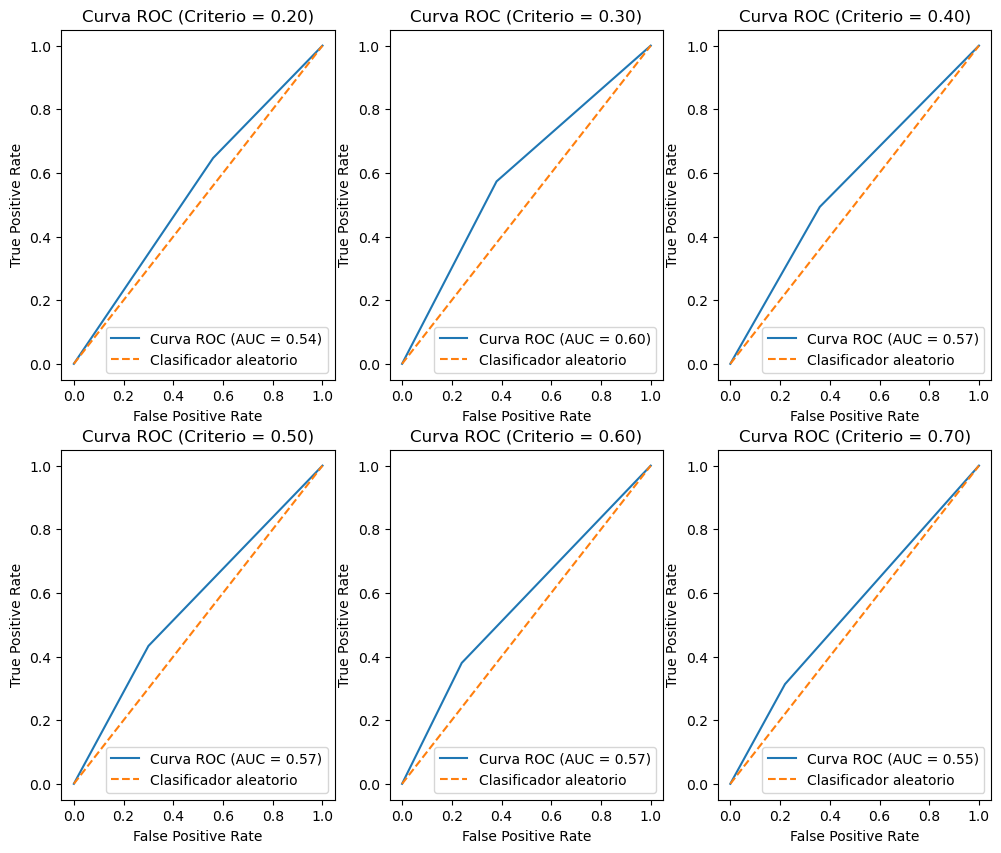
\includegraphics[width=1\textwidth]{img/curvasROC.PNG}
 \caption{Obtención del Mejor Criterio de Clasificación}
 \label{f:curvasROC}
\end{figure}

En tercer lugar, se ha separado una pequeña muestra de los datos originales: 150 registros de la clase NOK y 50 registros de la clase OK. De esta forma, se consigue que ningún modelo haya trabajado antes con estos datos y se puedan evaluar los modelos de una manera más aproximada

En este momento ya se contaba con todo listo para poder realizar diferentes experimentos para construir diferentes conjuntos de modelos, cambiando los parámetros que permiten construir las diferentes redes neuronales para obtener los mejores. Para todos los experimentos se ha seguido la siguiente estrategia:

\begin{itemize}
    \item \textbf{Capa convolucional:} esta capa o capas, según las que se le indiquen, junto con el \emph{kernel} indicado y su activación tipo \emph{relu}, aplican la técnica de convolución a los datos de entrada.
    \item \textbf{Pooling:} aplica la técnica \emph{pooling} y devuelve el valor máximo.
    \item \textbf{Flatten:} transforma los datos de entrada en un vector unidimensional.
    \item \textbf{Dense:} capa o capas que contienen el número de neuronas indicado junto con una activación tipo \emph{relu}.
\end{itemize}

Además, a la hora de entrenar el modelo, se ha utilizado un \emph{checkpoint} para quedarse con el modelo que menor \emph{loss} tenga. También, se pueden modificar el número de iteraciones durante el entreno.

Todo esto aplicando la técnica de validación cruzada y construyendo 5 modelos en cada experimento. Por lo que a la hora de obtener predicciones se sumará la predicción de los 5 modelos y se dividirá entre 5, y finalmente este valor se comparará con el criterio de clasificación, 0.3, y se determinará la clase de la bobina en concreto.

A continuación se recogen los resultados obtenidos tanto para los datos 1D como 2D, y para cada uno de ellos, los resultados obtenidos según si se utiliza solo el mapa codificado de la bobina, o el mapa junto con los demás atributos normalizados.

\subsubsection{Datos 1D}
Se han realizado un total de 7 experimentos para los datos 1D sobre el mapa codificado de la bobina. Los resultados han sido los siguientes:

\begin{itemize}
    \item \textbf{Experimento 1:} en este caso los parámetros utilizados han sido una capa convolucional con 32 filtros , el tamaño de \emph{kernel} es 3, 300 iteraciones, y tres capas densas de tamaños, respectivamente, 32, 8 y 1. Los resultados obtenidos son los siguientes:
    \begin{verbatim}
        La precisión obtenida ha sido 0.535
        La matriz de confusion obtenida es:
         [[27 23]
         [70 80]]
    \end{verbatim}
    \item \textbf{Experimento 2:} en este segundo experimento se han empleado una capa convolucional con 64 filtros y con un \emph{kernel} de tamaño 5. Las iteraciones han sido 500, y las capas densas se han mantenido iguales que en el caso anterior. Los resultados son los siguientes:
    \begin{verbatim}
        La precisión obtenida ha sido 0.54
        La matriz de confusion obtenida es:
         [[30 20]
         [72 78]]
    \end{verbatim}
    \item \textbf{Experimento 3:} en este tercer caso se ha usado una capa convolucional con 16 filtros y con un \emph{kernel} de tamaño 3. Las iteraciones han sido 300, y se han usado 5 capas densas de tamaños 64, 32, 16, 8 y 1. El resultado obtenido ha sido:
    \begin{verbatim}
        La precisión obtenida ha sido 0.54
        La matriz de confusion obtenida es:
         [[29 21]
         [71 79]]
    \end{verbatim}
    \item \textbf{Experimento 4:} en este cuarto caso se ha usado una capa convolucional de 16 filtros y con un \emph{kernel} de tamaño 5. Las iteraciones han sido 300 y se han empleado 3 capas densas de tamaño 32, 8 y 1.  Los resultados obtenidos han sido los siguientes:
    \begin{verbatim}
        La precisión obtenida ha sido 0.56
        La matriz de confusion obtenida es:
         [[29 21]
         [67 83]]
    \end{verbatim}
    \item \textbf{Experimento 5:} en este quinto experimento se han usado 3 capas convolucionales con  16, 32 y 64 filtros y todas ellas con un \emph{kernel} de tamaño 3. Las iteraciones y las capas densas han sido las mimas que las del experimento anterior. Los resultados obtenidos han sido;
    \begin{verbatim}
        La precisión obtenida ha sido 0.57
        La matriz de confusion obtenida es:
         [[32 18]
         [68 82]]
    \end{verbatim}
    \item \textbf{Experimento 6:} en este penúltimo experimento se han mantenido los valores del experimento anterior pero aumentando las iteraciones a 500. Los resultados han sido:
    \begin{verbatim}
        La precisión obtenida ha sido 0.56
        La matriz de confusion obtenida es:
         [[30 20]
         [68 82]]
    \end{verbatim}
    \item \textbf{Experimento 7:} en el último caso se han utilizado los mismos valores que en el experimento 5 pero cambiando el tamaño del \emph{kernel} a 5. Los resultados han sido:
    \begin{verbatim}
        La precisión obtenida ha sido 0.505
        La matriz de confusion obtenida es:
         [[26 24]
         [75 75]]
    \end{verbatim}
\end{itemize}

Sobre el mapa codificado y los atributos normalizados se han realizado otros 7 experimentos, cuyos resultados son los siguientes (en los resultados se incluye la precisión utilizando únicamente el modelo y la precisión obtenida combinando los modelos con el \emph{Random Forest}):

\begin{itemize}
    \item \textbf{Experimento 1:} este primer experimento ha sido con una capa convolucional con 32 filtros y con un \emph{kernel} de tamaño 3. Además, ternía 300 iteraciones y 3 capas densas de tamaños 32, 8 y 1. Los resultados han sido:
    \begin{verbatim}
        La precisión obtenida ha sido 0.47
        La matriz de confusion obtenida es:
         [[35 15]
         [91 59]]
        
        La precisión obtenida con el RF ha sido 0.475
        La matriz de confusion obtenida es:
         [[38 12]
         [93 57]]
    \end{verbatim}
    \item \textbf{Experimento 2:} este segundo caso ha sido igual que el anterior pero con un \emph{kernel} de tamaño 5 y con 16 filtros. Los resultados se muestran a continuación:
    \begin{verbatim}
        La precisión obtenida ha sido 0.51
        La matriz de confusion obtenida es:
         [[33 17]
         [81 69]]
        
        La precisión obtenida con el RF ha sido 0.445
        La matriz de confusion obtenida es:
         [[38 12]
         [99 51]]
    \end{verbatim}
    \item \textbf{Experimento 3:} en este tercer experimento ha sido similar al anterior pero con 64 filtros. Los resultados han sido:
    \begin{verbatim}
        La precisión obtenida ha sido 0.485
        La matriz de confusion obtenida es:
         [[39 11]
         [92 58]]
        
        La precisión obtenida con el RF ha sido 0.46
        La matriz de confusion obtenida es:
         [[40 10]
         [98 52]]
    \end{verbatim}
    \item \textbf{Experimento 4:} este cuarto caso ha sido igual que el primero pero con 16 filtros. Los resultados son:
    \begin{verbatim}
        La precisión obtenida ha sido 0.525
        La matriz de confusion obtenida es:
         [[35 15]
         [80 70]]
        
        La precisión obtenida con el RF ha sido 0.47
        La matriz de confusion obtenida es:
         [[35 15]
         [91 59]]
    \end{verbatim}
    \item \textbf{Experimento 5:} este quinto experimento ha sido igual que el anterior, solo que con 5 capas densas y de tamaños 64, 32, 16, 8 y 1. Se han obtenido los siguientes resultados:
    \begin{verbatim}
        La precisión obtenida ha sido 0.475
        La matriz de confusion obtenida es:
         [[34 16]
         [89 61]]
        
        La precisión obtenida con el RF ha sido 0.455
        La matriz de confusion obtenida es:
         [[40 10]
         [99 51]]
    \end{verbatim}
    \item \textbf{Experimento 6:} este penúltimo experimento ha sido igual que el anterior, pero con dos capas convolucionales con 32 y 64 filtros. Los resultados son:
    \begin{verbatim}
        La precisión obtenida ha sido 0.48
        La matriz de confusion obtenida es:
         [[31 19]
         [85 65]]
        
        La precisión obtenida con el RF ha sido 0.455
        La matriz de confusion obtenida es:
         [[31 19]
         [90 60]]
    \end{verbatim}
    \item \textbf{Experimento 7:} en el último caso, muy parecido al anterior, solo que con un \emph{kernel} de tamaño 5, se han obtenido los siguientes resultados:
    \begin{verbatim}
        La precisión obtenida ha sido 0.425
        La matriz de confusion obtenida es:
         [[ 39  11]
         [104  46]]
        
        La precisión obtenida con el RF ha sido 0.435
        La matriz de confusion obtenida es:
         [[ 43   7]
         [106  44]]
    \end{verbatim}
\end{itemize}

\subsubsection{Datos 2D}
Con respecto a los datos 2D, también se han realizado 7 experimentos sobre los mapas codificados de las bobinas. A continuación se muestran los resultados:

\begin{itemize}
    \item \textbf{Experimento 1:} en este primer caso se utiliza una capa convolucional con 32 filtros y un \emph{kernel} de tamaño 3x3. Además, se efectúan 100 iteraciones y tres capas densas de tamaños 32, 8 y 1. Los resultados han sido los siguientes:
    \begin{verbatim}
        La precisión obtenida ha sido 0.485
        La matriz de confusion obtenida es:
         [[37 13]
         [90 60]]
    \end{verbatim}
    \item \textbf{Experimento 2:} este experimento es muy similar al anterior, solo que con 16 filtros. Los resultados son los siguientes:
    \begin{verbatim}
        La precisión obtenida ha sido 0.49
        La matriz de confusion obtenida es:
         [[37 13]
         [89 61]]
    \end{verbatim}
    \item \textbf{Experimento 3:} este tercer caso es muy similar al primero, pero ahora el tamaño del \emph{kernel} es de 5x5. Sus resultados han sido:
    \begin{verbatim}
        La precisión obtenida ha sido 0.525
        La matriz de confusion obtenida es:
         [[34 16]
         [79 71]]
    \end{verbatim}
    \item \textbf{Experimento 4:} este tercer experimento es similar al primero, pero con 64 filtros. Además, tiene 5 capas densas de tamaños 64, 32, 16, 8 y 1. Sus resultados han sido:
    \begin{verbatim}
        La precisión obtenida ha sido 0.53
        La matriz de confusion obtenida es:
         [[41  9]
         [85 65]]
    \end{verbatim}
    \item \textbf{Experimento 5:} este experimento ha sido similar al primero, solo que con 16 filtros y un \emph{kernel} de tamaño 5x5. Los resultados han sido:
    \begin{verbatim}
        La precisión obtenida ha sido 0.495
        La matriz de confusion obtenida es:
         [[38 12]
         [89 61]]
    \end{verbatim}
    \item \textbf{Experimento 6:} este caso ha sido similar al primero pero con dos capas convolucionales con 16 y 32 filtros. Sus resultados han sido:
    \begin{verbatim}
        La precisión obtenida ha sido 0.49
        La matriz de confusion obtenida es:
         [[36 14]
         [88 62]]
    \end{verbatim}
    \item \textbf{Experimento 7:} este experimento ha sido similar al anterior, pero en este caso con tres capas convolucionales, de tamaños 16, 32 y 64. Los resultados han sido:
    \begin{verbatim}
        La precisión obtenida ha sido 0.54
        La matriz de confusion obtenida es:
         [[34 16]
         [76 74]]
    \end{verbatim}
\end{itemize}

Para los datos 2D juntando el mapa con los demás atributos, se han realizado de igual manera 7 experimentos. Además, al igual que para los datos 1D, se han añadido los resultados de usar \emph{Random Forest}. Todos los resultados se pueden ver a continuación:
\begin{itemize}
    \item \textbf{Experimento 1:} en este primer experimento se utiliza una capa convolucional con 32 filtros y un \emph{kernel} de 3x3. Además, se han empleado 100 iteraciones y 3 capas densas de tamaño 32, 8 y 1. Sus resultados han sido: 
    \begin{verbatim}
        La precisión obtenida ha sido 0.51
        La matriz de confusion obtenida es:
         [[41  9]
         [89 61]]
        
        La precisión obtenida con el RF ha sido 0.5
        La matriz de confusion obtenida es:
         [[42  8]
         [92 58]]
    \end{verbatim}
    \item \textbf{Experimento 2:} este segundo experimento ha sido similar al anterior, pero con 16 filtros y el \emph{kernel} de tamaño 5x5. Los resultados han sido:
    \begin{verbatim}
        La precisión obtenida ha sido 0.505
        La matriz de confusion obtenida es:
         [[30 20]
         [79 71]]
        
        La precisión obtenida con el RF ha sido 0.53
        La matriz de confusion obtenida es:
         [[39 11]
         [83 67]]
    \end{verbatim}
    \item \textbf{Experimento 3:} este caso ha sido muy similar al primero pero con un \emph{kernel} de 5x5. Los resultados han sido:
    \begin{verbatim}
        La precisión obtenida ha sido 0.525
        La matriz de confusion obtenida es:
         [[34 16]
         [79 71]]
        
        La precisión obtenida con el RF ha sido 0.51
        La matriz de confusion obtenida es:
         [[42  8]
         [90 60]]
    \end{verbatim}
    \item \textbf{Experimento 4:} este experimento ha sido como el primero, pero esta vez utilizando 16 filtros. Sus resultados han sido:
    \begin{verbatim}
        La precisión obtenida ha sido 0.49
        La matriz de confusion obtenida es:
         [[40 10]
         [92 58]]
        
        La precisión obtenida con el RF ha sido 0.47
        La matriz de confusion obtenida es:
         [[43  7]
         [99 51]]
    \end{verbatim}
    \item \textbf{Experimento 5:} este experimento ha sido similar al primero, pero las capas densas pasan a ser 5 y sus tamaños son 64, 32, 16, 8 y 1. Sus resultados son:
    \begin{verbatim}
        La precisión obtenida ha sido 0.515
        La matriz de confusion obtenida es:
         [[38 12]
         [85 65]]
        
        La precisión obtenida con el RF ha sido 0.495
        La matriz de confusion obtenida es:
         [[37 13]
         [88 62]]
    \end{verbatim}
    \item \textbf{Experimento 6:} en este sexto caso, similar al primero, se han añadido dos capas convolucionaales con 32 y 16 filtros. Los resultados son:
    \begin{verbatim}
        La precisión obtenida ha sido 0.51
        La matriz de confusion obtenida es:
         [[35 15]
         [83 67]]
        
        La precisión obtenida con el RF ha sido 0.515
        La matriz de confusion obtenida es:
         [[42  8]
         [89 61]]
    \end{verbatim}
    \item \textbf{Experimento 7:} este experimento ha sido similar al anterior, pero con una capa convolucional más. Sus tamaños son 16, 32 y 64, y cuyos resultados son:
    \begin{verbatim}
        La precisión obtenida ha sido 0.49
        La matriz de confusion obtenida es:
         [[39 11]
         [91 59]]
        
        La precisión obtenida con el RF ha sido 0.475
        La matriz de confusion obtenida es:
         [[42  8]
         [97 53]]
    \end{verbatim}
\end{itemize}

\subsubsection{Análisis de resultados}
Para concluir con esta fase, es turno de analizar los resultados que se han obtenido, y que han sido mostrados en los dos subpuntos anteriores.

Lo primero que resalta son los malos resultados, ya que ninguno de los 28 experimentos han mostrado una precisión adecuada, de hecho, casi todos están con una precisión de entre el 50 y 60 porciento, unos resultados para nada aceptables.

Si comparamos los resultados entre los datos 1D y 2D, se ve como las precisiones más altas son las del primer tipo de datos, algo que puede chocar, ya que se puede presuponer que los datos 2D mostrarán algún patrón o característica que haga que el modelo sea mejor, pero no ha sido el caso. Es por ello, que se cree que esto se debe a que en los datos prestados el operario usa para clasificar las bobinas los datos 1D, de ahí esos posibles mejores resultados.

Si comparamos los resultados obtenidos directamente con los modelos a los obtenidos por el \emph{random forest}, se ve como este último, casi siempre es similar o un poco peor que si utilizamos solo el modelo, por lo que no muestra ningún síntoma de ser beneficioso su uso.

Finalmente, el mejor resultado, se ha obtenido con el experimento 5 de los datos 1D empleando tan solo el mapa codificado de la bobina, por lo que será este el que se empleará en la siguiente fase.

\section{Desarrollo de la Aplicación}
En esta sexta y última fase, ha sido turno de construir la aplicación final del proyecto, sobre la cual se puedan cargar datos de bobinas medidos por sensores y predecir y si serán bobinas válidas o no. 

La construcción de la aplicación se ha basado en dos partes. Por un lado, tenemos un \emph{notebook} donde se podrá elegir la base de datos donde se encuentran los datos y visualizar los resultados. Y, por otro lado, tenemos un archivo de \emph{Python} que contiene las diferentes funciones y que encapsula, de cara al usuario, todo el proceso, con el fin de dejar la aplicación lo vas sencilla y visual posible. 

Con respecto a los modelos usados para las predicciones, se han correspondido a los del experimento 5 sobre los datos 1D, ya que, como ya se ha visto en la fase anterior, han sido los que mejores resultados han dado. 

Además, para añadirle más funcionalidad a la aplicación, cada vez que se realizan predicciones sobre un modelo, se genera un archivo CSV que contiene todas las características obtenidas de la bobina, puesto que puede ser interesante almacenar los valores por si fuesen de utilidad al operario. Y también, se ha creado un histórico donde se almacenan las predicciones de las bobinas para poder consultarlas en el futuro sin la necesidad de tener que volver a cargar los datos.

El resultado se puede ver en la Figura \ref{f:apli1}, donde se aprecia la tabla con las diferentes \emph{features} calculadas y el mapa codificado de la bobina. Además, más abajo se puede ver la predicción obtenida por los modelos según los datos obtenidos por cada par de sensores.

\begin{figure}[h]
 \centering
  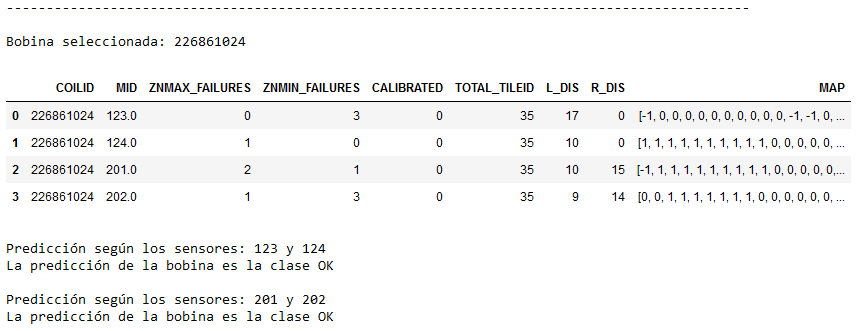
\includegraphics[width=1\textwidth]{img/salidaAp.PNG}
 \caption{Ejemplo de Resultado de la Aplicación}
 \label{f:apli1}
\end{figure}

Y como se ha comentado, se ha generado a su vez un archivo CSV con todos los atributos calculados de la bobina y su mapa codificado para cada sensor. La Figura \ref{f:apli2}, muestra el CSV generado para la bobina de ejemplo mostrada en la imagen anterior. 

\begin{figure}[h]
 \centering
  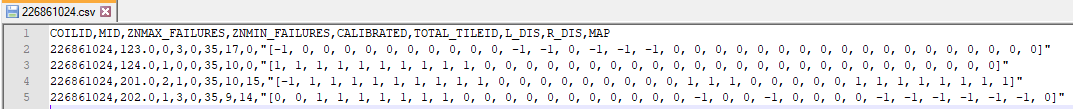
\includegraphics[width=1\textwidth]{img/csv.PNG}
 \caption{Ejemplo de Resultado del CSV Genrado por la Aplicación}
 \label{f:apli2}
\end{figure}

Y también se ha generado un archivo historial.txt que contiene el registro de predicciones. La Figura \ref{f:apli3}, muestra dicho resultado. 

\begin{figure}[h]
 \centering
  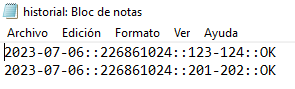
\includegraphics[width=0.5\textwidth]{img/historial.PNG}
 \caption{Ejemplo de Resultado del histroial.txt Genrado por la Aplicación}
 \label{f:apli3}
\end{figure}

Además, si siguiéramos realizando predicciones, se generaría un CSV correspondiente a la bobina y en el fichero correspondiente al historial se añadirían al final la nueva información.
\capitulo{7}{Conclusiones y Líneas de trabajo futuras}

\section{Conclusiones}
Tras la investigación llevada a cabo en este proyecto, los resultados obtenidos, al aplicar redes neuronales convolucionales sobre los datos prestados a la empresa, no han sido los deseados, ya que la mayor precisión obtenida ha sido del 57\%, un valor para nada aceptable.

Es por ello, que creemos que al contar con un conjunto desbalanceado y con, tal vez, pocos ejemplos, los resultados no han sido tan buenos como los que cabría esperar. Además, es probable que este tipo de red neuronal no sea la mejor ante los datos de entrada. Por lo que, consideramos que si se consiguen más datos, y quizás con un nuevo enfoque, se puedan obtener precisiones aceptables por parte de la empresa.

Finalmente, y como es obvio, no se está satisfecho con los resultados obtenidos, aunque pensamos que se han seguido buenas estrategias frente a los datos prestados. Por todo lo anterior, en el siguiente apartado se plantean varias propuestas para mejorar los módelos y conseguir resultados más precisos. 

\section{Líneas de trabajo futuras}
Bajo mi punto de vista, creo que los siguientes pasos y mejoras del proyecto son:
\begin{enumerate}
    \item \textbf{Aumento de bobinas clasificadas pertenecientes a la clase NOK}: con el fin de tener un conjunto de datos más equilibrado y poder crear mejores modelos, sería interesante obtener más bobinas pertenecientes a la clase NOK. De igual manera, si el número de bobinas pertenecientes a la clase OK también aumenta, es bastante posible que el modelo obtenido sea más preciso. En definitiva, cuantos más datos se posean y más equitativo sea el conjunto de datos, los resultados que se consigan serán seguramente mejores.
    \item \textbf{Conocer de manera exacta los criterios de validación de las bobinas:} como ya se ha comentado previamente, la empresa no nos ha dicho en ningún momento cuáles son los criterios exactos que usan para dar como válida o no una bobina, sino que simplemente con los datos medidos nos han pedido que creemos un modelo que sea capaz de aprender y realizar predicciones. Es por ello, que si se supieran sus criterios, se podría ajustar de alguna forma el modelo o utilizar alguna otra herramienta que mejore y facilite las predicciones.
    \item \textbf{Desarrollar una aplicación web:} la aplicación actual es un \emph{notebook} sobre el cual se pueden cargar bobinas y con los modelos generados realizar predicciones sobre si serán válidas o no. Pero su interfaz no es del todo amigable, sobre todo para gente que no haya hecho nunca programación y es necesario tener en ejecución el archivo para poder utilizarlo. Es por ello, que sería una gran mejora hacer la aplicación en un entorno web con una interfaz sencilla para que los operarios puedan emplearla fácilmente.
\end{enumerate}



%\renewcommand\chaptername{Anexo}
%\renewcommand\thechapter{\Roman{chapter}}
%\setcounter{chapter}{0}

% Añadir entrada en el índice: Anexos
\appendix
\addcontentsline{toc}{part}{Apéndices}
\part*{Apéndices}

\apendice{Plan de Proyecto Software}

\section{Introducción}

\section{Planificación temporal}

\section{Estudio de viabilidad}

\subsection{Viabilidad económica}

\subsection{Viabilidad legal}



\apendice{Especificación de Requisitos}

\section{Introducción}
Este segundo apéndice recuerda los objetivos generales marcados en el proyecto, y que previamente se han comentado en la memoria. Además tratará el catálogo de requisitos junto con su especificación y diagramas de caso de uso.

\section{Objetivos generales}
El proyecto se ha maracdo los siguientes objetivos generales:
\begin{itemize}
    \item Ayudar a la empresa que origina el proyecto, consiguiendo que se puedan identificar el mayor número de bobinas con errores aprovechables por parte de la empresa.
    \item Aumentar la eficiencia de la cadena de galvanizado de la empresa, de manera que un operario no tenga que analizar de forma exhaustiva cada bobina, para saber si es utilizable o no.
    \item Crear una cadena más sostenible, consiguiendo que se puedan aprovechar al máximo las bobinas galvanizadas y evitar que se tenga que desperdiciar demasiado material.   
\end{itemize}

\section{Catalogo de requisitos}
A continuación se indican los requisitos marcados en la aplicación llevada a cabo en el proyecto:
\begin{itemize}
    \item \textbf{REQ 1:} conseguir una aplicación capaz de ejecutar un conjunto de modelos sobre los datos de una bobina.
    \begin{itemize}
        \item \textbf{REQ 1.1:} cargar los datos medidos por los sensores.
        \item \textbf{REQ 1.2:} obtener las principales características de las bobinas.
        \item \textbf{REQ 1.3:} evaluar las bobinas con los modelos.
        \item \textbf{REQ 1.4:} mostrar si la bobina es válida o no.
    \end{itemize}
     \item \textbf{REQ 2:} permitir que los resultados obtenidos puedan descargarse.
    \begin{itemize}
        \item \textbf{REQ 2.1:} descargar las características obtenidas de las bobinas.
        \item \textbf{REQ 2.2:} descargar los rsultados obtenidos por el modelo.
    \end{itemize}
    \item \textbf{REQ 3:} generar un archivo que contenga el historial de las diferentes bobinas cargadas y evaluadas.
        \begin{itemize}
            \item \textbf{REQ 3.1:} guardar en el fichero el día en que se cargó la bobina, junto con la clase predicha.
        \end{itemize}
\end{itemize}

\section{Especificación de requisitos}
\subsection{Actores}
En esta aplicación tan solo se detecta un actor: el operario de la empresa. Ya que es el encargado, una vez se cuenten con los datos obtenidos por los sensores sobre la bobina, de dirigirse a la aplicación y realizar la predicción sobre los mismos.

\newpage
\subsection{Diagrama de casos de uso}
La Figura \ref{f:casus} muestra el diagrama de casos de uso de la aplicación.

\begin{figure}[h]
 \centering
  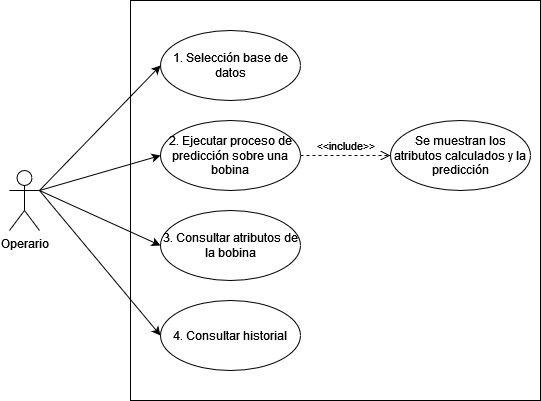
\includegraphics[width=1\textwidth]{img/casosUso.png}
 \caption{Diagrama de Casos de Uso}
 \label{f:casus}
\end{figure}

\newpage
\subsection{Especificación de casos de uso}
A continaucón se muestra una tabla para cada caso de uso:

\begin{center}
\begin{tabular}{|ll|}
\hline
\multicolumn{2}{|l|}{\textbf{CU 1 - Selección base de datos}}                                                                                                                                                          \\ \hline
\multicolumn{1}{|l|}{\textbf{Descripción}}     & \begin{tabular}[c]{@{}l@{}}Permite al operario seleccionar los diferentes valores que \\ permitan conectarse a la base de datos para cargar los valores.\end{tabular} \\ \hline
\multicolumn{1}{|l|}{\textbf{Requisitos}}      & REQ 1.1                                                                                                                                                               \\ \hline
\multicolumn{1}{|l|}{\textbf{Precondiciones}}  & Se está ejecutando el notebook de la aplicación.                                                                                                                      \\ \hline
\multicolumn{1}{|l|}{\textbf{Secuencia}}       & \begin{tabular}[c]{@{}l@{}}1. El usuario rellena los campos: user, password, host y \\ database \\ 2. El usuario ejecuta la celda correspondiente\end{tabular}            \\ \hline
\multicolumn{1}{|l|}{\textbf{Postcondiciones}} & La celda se ejecuta bien y aparece un 2 a su izquierda                                                                                                                \\ \hline
\multicolumn{1}{|l|}{\textbf{Excepciones}}     & \begin{tabular}[c]{@{}l@{}}Se introducen los valores de forma incorrecta y sin el formato \\ necesario en Python y salta un error\end{tabular}                        \\ \hline
\end{tabular}
\captionof{table}{Caso de Uso - 1}
\label{t:caso1}
\end{center}

\begin{center}
\begin{tabular}{|ll|}
\hline
\multicolumn{2}{|l|}{\textbf{CU 2 - Ejecución proceso de predicción sobre una bobina}}                                                                                                                                                                                                                                \\ \hline
\multicolumn{1}{|l|}{\textbf{Descripción}}     & \begin{tabular}[c]{@{}l@{}}Permite al operario seleccionar la ID de la bobina desea\\ sobre la que calcular las predicciones.\end{tabular}                                                                                                                           \\ \hline
\multicolumn{1}{|l|}{\textbf{Requisitos}}      & REQ 1.2, REQ 1.3 y REQ 1.4                                                                                                                                                                                                                                           \\ \hline
\multicolumn{1}{|l|}{\textbf{Precondiciones}}  & \begin{tabular}[c]{@{}l@{}}Se está ejecutando el notebook de la aplicación, y se\\ ha indicado la base de datos.\end{tabular}                                                                                                                                        \\ \hline
\multicolumn{1}{|l|}{\textbf{Secuencia}}       & \begin{tabular}[c]{@{}l@{}}1. El usuario ejecuta la tercera celda.\\ 2. El usuario selecciona en el desplegable la ID de la\\ bobina.\\ 3. El usuario observa los valores y predicciones mostradas\\ por pantalla, y decide si seleccionar otra bobina.\end{tabular} \\ \hline
\multicolumn{1}{|l|}{\textbf{Postcondiciones}} & \begin{tabular}[c]{@{}l@{}}Se muestran los atributos calculados de la bobina y \\ la decisión del modelo.\end{tabular}                                                                                                                                               \\ \hline
\multicolumn{1}{|l|}{\textbf{Excepciones}}     & \begin{tabular}[c]{@{}l@{}}Se produce algún problema durante el proceso y el \\ modelo devuelve algún error.\end{tabular}                                                                                                                                            \\ \hline
\end{tabular}
\captionof{table}{Caso de Uso - 2}
\label{t:caso2}
\end{center}

\begin{center}
\begin{tabular}{|ll|}
\hline
\multicolumn{2}{|l|}{\textbf{CU 3 - Consultar atributos de la bobina}}                                                                                                                                                                                                                  \\ \hline
\multicolumn{1}{|l|}{\textbf{Descripción}}     & \begin{tabular}[c]{@{}l@{}}Permite al operario conocer los atributos y el mapa\\ codificado de la bobina previamente calculados.\end{tabular}                                                                                          \\ \hline
\multicolumn{1}{|l|}{\textbf{Requisitos}}      & REQ 2.1                                                                                                                                                                                                                                \\ \hline
\multicolumn{1}{|l|}{\textbf{Precondiciones}}  & Se ha realizado una predicción sobre la bobina deseada.                                                                                                                                                                                \\ \hline
\multicolumn{1}{|l|}{\textbf{Secuencia}}       & \begin{tabular}[c]{@{}l@{}}1. El usuario se dirige a la ruta donde se encuentra\\ la aplicación.\\ \\ 2. El usuario se dirige al directorio /bobinas.\\ 3. El usuario abre el CSV correspondiente a la \\ bobina deseada.\end{tabular} \\ \hline
\multicolumn{1}{|l|}{\textbf{Postcondiciones}} & \begin{tabular}[c]{@{}l@{}}El usuario consigue abrir el fichero correctamente, y\\ en su interior se encuentran todos los atributos.\end{tabular}                                                                                      \\ \hline
\multicolumn{1}{|l|}{\textbf{Excepciones}}     & -                                                                                                                                                                                                                                      \\ \hline
\end{tabular}
\captionof{table}{Caso de Uso - 3}
\label{t:caso3}
\end{center}

\begin{center}
\begin{tabular}{|ll|}
\hline
\multicolumn{2}{|l|}{\textbf{CU 4 - Consultar el historial}}                                                                                                                                                  \\ \hline
\multicolumn{1}{|l|}{\textbf{Descripción}}     & \begin{tabular}[c]{@{}l@{}}Permite al operario poder revisar el historial de las\\ diferentes predicciones realizadas.\end{tabular}                          \\ \hline
\multicolumn{1}{|l|}{\textbf{Requisitos}}      & REQ 2.2 y REQ 3                                                                                                                                              \\ \hline
\multicolumn{1}{|l|}{\textbf{Precondiciones}}  & \begin{tabular}[c]{@{}l@{}}Se ha realizado al menos una predicción sobre\\ cualquier bobina.\end{tabular}                                                    \\ \hline
\multicolumn{1}{|l|}{\textbf{Secuencia}}       & \begin{tabular}[c]{@{}l@{}}1. El usuario se dirige a la ruta donde se encuentra\\ la aplicación.\\ 2. El usuario sabre el archivo historial.txt\end{tabular} \\ \hline
\multicolumn{1}{|l|}{\textbf{Postcondiciones}} & \begin{tabular}[c]{@{}l@{}}El archivo contiene en su interior los resultados\\ previamente calculados.\end{tabular}                                          \\ \hline
\multicolumn{1}{|l|}{\textbf{Excepciones}}     & -                                                                                                                                                            \\ \hline
\end{tabular}
\captionof{table}{Caso de Uso - 4}
\label{t:caso4}
\end{center}
\apendice{Especificación de diseño}

\section{Introducción}

\section{Diseño de datos}

\section{Diseño procedimental}

\section{Diseño arquitectónico}



\apendice{Documentación técnica de programación}

\section{Introducción}
Este cuarto apéndice va destinado a las personas dedicadas a la informática y que quieran seguir con el proyecto en el futuro. Es por ello, que es necesario explicar todo claramente para que se pueda comprender. Los temas sobre los que se va a tratar son: estructura de directorios, manual del programador, ejecución del proyecto y pruebas del sistema.

\section{Estructura de directorios}
Este subapartado contiene la información sobre la estructura del proyecto, junto con sus diferentes directorios y ficheros. Además, toda la estructura se puede ver de manera pública en el repositorio de GitHub\footnote{Repositorio: \url{https://github.com/ifh1001/TFM}} del proyecto. A continuación, se puede ver de manera gráfica:
\dirtree{%
.1 /.
.2 \texttt{doc}.
.2 \texttt{src}.
.2 \texttt{LICENSE}.
.2 \texttt{README.md}.
.2 \texttt{requirements.txt}.
}
Como se aprecia, se distinguen del directorio raíz 5 elementos, que se van a explicar a continuación:
\begin{itemize}
    \item \textbf{doc:} contiene toda la información relacionada con la documentación.
    \item \textbf{src:} contiene en su interior todo el código desarrollado a lo largo del proyecto. Además, contiene la aplicación, junto con todo lo necesario para que pueda usarse.
    \item \textbf{LICENSE:} fichero que contiene la licencia del proyecto, que como ya se ha comentado en el primer apéndice, es una licencia de tipo GPL v3.
    \item \textbf{README.md:} contiene una breve descripción del repositorio, con el fin de que el lector comprenda la finalidad del proyecto.
    \item \textbf{requirements.txt:} fichero que reúne los requisitos necesarios de librerías y versiones para ejecutar sin ningún problema la aplicación.
\end{itemize}

\subsection{Documentación}
Como se ha comentado previamente, la documentación se encuentra en el directorio \texttt{/doc}. En él se encuentra un conjunto de ficheros escritos en \LaTeX que si se compilan todos ellos juntos se obtiene la memoria en formato PDF que da lugar a esta memoria que se está leyendo.

\subsection{Código}
El código desarrollado en el proyecto se encuentra en el directorio \texttt{/src}. A continuación se muestra la división de directorios y ficheros del mismo:
\dirtree{%
.1 \texttt{/src/}.
.2 \texttt{aplicacion}.
.3 \texttt{modelos}.
.3 \texttt{Aplicacion.ipynb}.
.3 \texttt{funciones.py}.
.2 \texttt{CargaDatos.ipynb}.
.2 \texttt{EvaluacionCNNs.ipynb}.
.2 \texttt{ObtencionCaracteristicas.ipynb}.
.2 \texttt{PreparacionCNNs.ipynb}.
.2 \texttt{VisualizacionDatos.ipynb}.
}

Como se puede apreciar, el directorio \texttt{/src} está formado por un directorio y cinco \emph{notebooks}. A continuación, se puede ver una explicación sobre cada uno:

\begin{itemize}
    \item \texttt{aplicacion:} en este directorio se encuentra la estructura necesaria para que funcione la aplicación. Como se puede ver, hay un directorio más, \texttt{/modelos}, donde se encuentran almacenados los cinco modelos que utilizará la aplicación. Además, hay dos ficheros, un \emph{notebook} que será la aplicación y un fichero de \emph{Python} que contiene todas las funciones de manera encapsulada para que se pueda utilizar la aplicación de la manera más sencilla posible.
    \item \texttt{CargaDatos.ipynb:} este \emph{notebook} contiene las primeras pruebas que se realizaron sobre los datos para conocer las diferentes tablas y registros que tenía cada una. Además, contiene una evaluación de bobinas según si cumplen o no todas sus tejas, los requisitos de zinc.
    \item \texttt{EvaluacionCNNs.ipynb:} este fichero contiene los diferentes experimentos que se han llevado a cabo para obtener él mejore conjunto de modelos con la mayor precisión. Además, también guarda todos los modelos obtenidos para poder emplear cualquiera.
    \item \texttt{ObtencionCaracteristicas.ipynb:} este \emph{notebook} se encarga de obtener el mapa codificado de cada bobina junto con las diferentes \emph{features}. Todos estos datos se calculan para cada tipo de datos, 1D y 2D, y para cada uno de los diferentes sensores.
    \item \texttt{PreparacionCNNs.ipynb:} este fichero contiene las diferentes pruebas que se han efectuado para aprender a construir modelos con \emph{tensorflow} para familiarizarse con la librería y sentirse cómodo con el uso de la misma.
    \item \texttt{VisualizacionDatos.ipynb:} contiene una visualización de los valores de zinc para cada bobina en forma de gráfica, para cada uno de los sensores de los datos 1D.
\end{itemize}

\section{Manual del programador}
Tal y como se acaba de ver en el subpunto anterior. La aplicación se encuentra en el directorio \texttt{/src/aplicacion}. En él se pueden implementar nuevas funcionalidades de la aplicación añadiéndolas al fichero \texttt{funciones.py}. Además, en su interior, se encuentran todas las funciones debidamente comentadas para que puedan ser comprendidas y mejoradas en caso de que se desee. Adicionalmente, si se consiguen mejores modelos se pueden eliminar los antiguos y añadir los nuevos en el directorio \texttt{/src/aplicacion/modelos}.

Si se quiere realizar alguna prueba más sobre las redes neuronales, o construir algunas nuevas empleando diferentes estrategias, o incluso utilizando datos diferentes, mi recomendación es que se realice en un \emph{notebook}, usando por ejemplo \emph{Jupyter Notebook}, ya que permite visualizar todo de una manera mucho más sencilla y posteriormente exportar las funciones a un fichero de \emph{Python}. Todos estos nuevos ficheros se pueden añadir directamente al directorio raíz del código (\texttt{/src}).

\section{Compilación, instalación y ejecución del proyecto}
Para usar la aplicación desarrollada en el proyecto, es necesario tener instalado en el dispositivo un entorno que tenga todas las dependencias de librerías que usa la aplicación, junto con una herramienta que permita ejecutar \emph{notebooks}, siendo recomendad el uso de \emph{Jupyter Notebook}.

Las librerías utilizadas se pueden ver a continuación:
\begin{itemize}
    \item MySQL
    \item Pandas
    \item NumPY
    \item Jupyter Widgets
    \item TensorFlow
\end{itemize}

De forma que al instalar todas ellas en un entorno, se podría ejecutar sin ningún problema la aplicación. Pese a todo, y por si en algún punto existen versiones incompatibles entre sí, en el repositorio de GitHub existe el fichero \texttt{requirements.txt} para que se puedan instalar en un entorno de Anaconda las versiones utilizadas en el proyecto que garantizarían el correcto empleo de la aplicación. Dicho fichero se puede encontrar en el siguiente enlace:

\url{https://github.com/ifh1001/TFM/blob/main/requirements.txt}

Una vez se cuenten con las librerías instaladas, se puede usar la aplicación. Para ello, con una herramienta que permita ejecutar \emph{notebooks} se puede abrir el correspondiente a la aplicación y ejecutar las tres celdas que la componen para poder seleccionar las bobinas sobre las que realizar predicciones.

\section{Pruebas del sistema}
Este proyecto se ha centrado en la investigación de obtener un grupo de modelos capaces de predecir si una bobina iba a ser válida o no para poder usarse por parte de la empresa. Es por ello, que se ha dado más peso a la investigación que a la construcción de una aplicación lo más perfecta posible y realizando pruebas de sistema para garantizar su correcto funcionamiento.

Pese a todo, se han llevado a cabo dos pruebas relevantes a la hora de construir y evaluar los modelos. Por un lado, se han separado del conjunto de datos inicial, una muestra de bobinas para, tras construir los modelos, evaluarlos con datos que nunca habían visto y así obtener unos resultados lo más realistas y probables posibles.

Por otro lado, se llevó a cabo una prueba para obtener el mejor criterio de clasificación, probando un total de 6 valores, y para cada uno de ellos calcular y representar la curva ROC junto con su AUC, de forma, que se ha trabajado con aquel que mejor AUC tenía, ya que este criterio es él más óptimo para separar las clasificaciones entre una clase u otra.
\apendice{Documentación de usuario}

\section{Introducción}
En este último apéndice, se incluye la información necesaria para poder utilizar la aplicación del proyecto, como poder instalarlo y el manual de usuario para saber utilizar la aplicación.

\section{Requisitos de usuarios}
El primer requisito por parte del usuario es la necesidad de tener conexión a Internet, ya que los datos se encuentran alojados en una base de datos, por lo que para poder usarla será necesario tener conexión.

En segundo lugar, necesitará tener un entorno con todas las librerías que usa la aplicación, junto con alguna aplicación que permite ejecutar un \emph{notebook}, como, por ejemplo, \emph{Jupyter Notebook}.

Una vez se diponga de todo lo anterior, ya sería posible poder utilizar la aplicación que se ha llevado a cabo en este proyecto.

\section{Instalación}
En primer lugar, sería necesario descargar en instalar Anaconda en caso de que no se disponga de dicha herramienta, ya que permite crear un entorno con todos los requisitos de la aplicación, permitiendo que se pueda usar sin ningún problema. Para ello, es tan sencillo como ir a la siguiente ruta:

\url{https://www.anaconda.com/download}

Y en ella descargar la versión adecuada a tu sistema operativo. Tras esto, sería tan sencillo como seguir el instalador y esperar unos minutos a que termine la instalación.

En segundo lugar, habría que instalar las dependencias de la aplicación. Para facilitar este proceso se ha dejado en el repositorio del proyecto un fichero \emph{requirements}, obtenido de un entorno \emph{Windows}, que permitirá descargar todas las librerías junto con sus versiones que hacen que se garantice la posibilidad de utilizar la aplicación. Dicho fichero se puede encontrar en el siguiente enlace:

\url{https://github.com/ifh1001/TFM/blob/main/requirements.txt}

En tercer, y último lugar, para poder instalar las dependencias, se abrirá la consola \emph{Anaconda Prompt} y se escribirá el siguiente comando:

\begin{verbatim}
conda create --name nombre_entorno --file requirements.txt
\end{verbatim}

Y tras esperar unos minutos, se habrán instalado todas las dependencias, por lo que ya se ha creado un entorno que sea capaz de lanzar la aplicación.

\section{Manual del usuario}
En primer paso para poder utilizar la aplicación, es lanzar \emph{Jupyter Notebook}. Para ello, y basándose en el apartado de instalación, lo primero sería cambiar al nuevo entorno, y posteriormente ejecutar el comando de la herramienta. Ambos comandos se muestran a continuación:

\begin{verbatim}
    conda activate nombre_entorno
    
    jupyter notebook
\end{verbatim}

Tras su ejecución aparecerá en el navegador la herramienta, y sería tan sencillo como dirigirse al directorio donde se encuentra el \emph{notebook} de la aplicación. Tras abrirlo se verá que hay 3 celdas y que habrá que ejecutar en orden. Para ejecutar una celda, hacemos clic sobre ella y pulsamos al botón \textbf{Run} que se encuentra en el menú superior, tras esperar un rato veremos como a la izquierda de la celda aparecerá un 1, de igual forma que se puede ver en la Figura \ref{f:celda1}.

\begin{figure}[h]
 \centering
  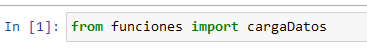
\includegraphics[width=0.7\textwidth]{img/celda1.PNG}
 \caption{Ejecución de la Primera Celda}
 \label{f:celda1}
\end{figure}

A continuación, será necesario ejecutar la segunda celda, o previamente modificar los valores en caso de que se quiera utilizar una base de datos diferente a la que viene por defecto. Tras su ejecución aparecerá a la izquierda un 2.

Finalmente, se ejecutará la última celda, y se verá como aparece un desplegable que muestra las IDs de todas las bobinas cargadas de la base de datos, Figura \ref{f:celda3}. Sería tan sencillo como seleccionar una y esperar a que aparezcan los resultados. Este proceso se puede repetir tantas veces como se desee, simplemente volviendo a seleccionar otra bobina desde el desplegable.

\begin{figure}[h]
 \centering
  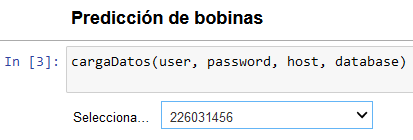
\includegraphics[width=0.7\textwidth]{img/celda3.PNG}
 \caption{Ejecución de la Tercera Celda}
 \label{f:celda3}
\end{figure}

También, en el directorio \texttt{./bobinas} se verán los diferentes CSV asociados a las bobinas sobre las que se han realizado predicciones. Además, junto al \emph{notebook} de la aplicación, se encontrará el fichero historial.txt donde se podrá consultar las predicciones de todas las bobinas.

Tras usar la aplicación, sería tan sencillo como cerrar la pestaña de la aplicación y finalmente cerrar la consola desde la que se ha lanzado \emph{Jupyter Notebook}, y de esta forma se detendría todo el proceso por completo.


\bibliographystyle{plain}
\bibliography{bibliografia}

\end{document}
